\begin{document}
The ring oscillator required that the capacitances be increased in order to create the correct output waveform. A 560pF and a 1.2nF capacitor were added in parallel with the ring oscillator capacitors. The output from the ring oscillator is shown in Figure \ref{fig:vringout}.

\begin{figure}[H]
	\centering
	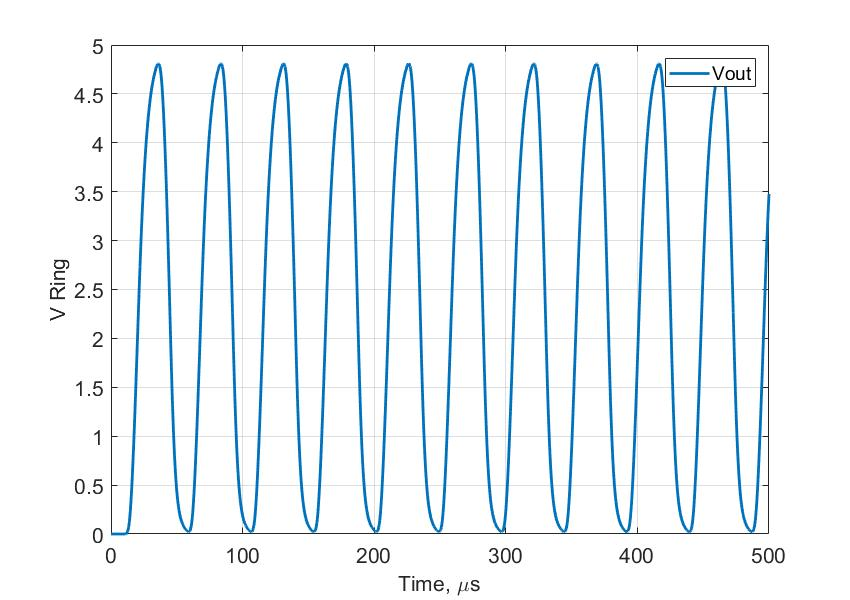
\includegraphics[width=0.6\linewidth]{ExperimentalImplementation/vring_out}
	\caption[Experimental ring output]{Experimental output of ring oscillator}
	\label{fig:vringout}
\end{figure}

The output wave form was 20.19kHz, with a duty-cycle of 50.03\%. The changes required by the circuit are summarized in Table \ref{tab:expvaluering}.

\begin{table}[H]
	\centering
	\caption{Ring oscillator comparisons}
	\label{tab:expvaluering}
	\begin{tabular}{|l|l|l|}
		\hline
		Component Values & Simulated & Experimental   \\ \hline
		C$_1$            & 8.2nF     & 8.2nF $||$ 560pF \\ \hline
		C$_2$            & 8.2nF     & 8.2nF $||$ 1.2nF \\ \hline
		C$_3$            & 8.2nF     & 8.2nF          \\ \hline
	\end{tabular}
\end{table}

After the required changes the circuit operated correctly.


\end{document}